\chapter{Methods}\label{chap:methods}
\begin{chapabstract}

%In this chapter, we describe procedures of our study from making a subsample of HRS galaxies to calculating the radio SFR\@.
In this Chapter, we describe procedures of our study from doing the fitting on $\qn$ to calculating the radio SFR\@.
Section~\ref{sec:tirluminosity} describes the method to estimate total IR luminosity from several IR bands' observations.
Section~\ref{sec:fittingtoq} shows how to find the frequency dependence of $\qn$ by the fitting.
Section~\ref{sec:calculatingsfr} describes how to calculate SFR from the low-frequency radio emission.

\end{chapabstract}

\section{Calculating the $\qn$ Parameter}\label{sec:calculatingq}
In this Section, we introduce the method to calculate the $\qn$ parameter, which shows the ratio between integrated IR and radio luminosities in a galaxy.
The definition of this parameter here is given on the following equation \citep[e.g.,][]{Helou1985, Bell2003, CalistroRivera2017a}:

\begin{equation}\label{eq:q_def}
    \qn \equiv \log\brp{\frac{L\msb{8-1000\,\mu m}\ /\ 3.75 \times 10^{12}}{{\rm erg\,s^{-1}\,Hz^{-1}}}} - \log\brp{\frac{L_{\mr{Radio},\,\nu}}{{\rm erg\,s^{-1}\,Hz^{-1}}}}
\end{equation}
where $L\msb{8-1000\,\mu m}$ is the total rest-frame infrared luminosity among $8 \mbox{--} 1000\,\mr{\mu m}$ and $3.75\times10^{12}\,\mr{Hz}$ is equivalent to the frequency of $80\,\mr{\mu m}$ for correcting the dimension.

Although \citet{Ciesla2014} have already derived the total IR luminosity for most HRS galaxies using the SED fitting, one of our galaxy samples (HRS163) does not have the value because of the lack of the reliable mid-IR flux from {\it Spitzer\/} telescope.
For consistency, we adopt the total IR luminosity calculated from the same method for all galaxy samples.
%To calculate the total IR luminosity, we refer to \citet{Galametz2013}, which derive the calibration relation between combining monochromatic IR luminosities and the total IR luminosity.
To calculate the total IR luminosity, we refer to \citet{Galametz2013}, which derives the calibration relation of the total IR luminosity with monochromatic IR luminosities.
We show the procedure to calculate total IR luminosity in the next Section.



\section{Total IR Luminosity}\label{sec:tirluminosity}
In this Section, we present how to calculate the total IR luminosity in this study.
For the method of calculating total IR luminosity, we refer to \citet{Galametz2013}, which shows the empirical relations to estimate total IR from {\it Spitzer\/} ($24, 70\micron$) and {\it Herschel\/} bands ($100, 160, 250\micron$).
HRS galaxies have flux data from the Multiband Imaging Photometry for {\it Spitzer\/} (MIPS;~\citealt{Rieke2004, Bendo2012}), the {\it Herschel\/}/PACS ($100,\,160\micron$; \citealt{Cortese2014c}) and the {\it Herschel\/}/SPIRE ($250\micron$; \citealt{Ciesla2012a}).

\citet{Galametz2013} derived the calibration equation below:

\begin{equation}\label{eq:galametz}
    L\msb{3-1100\mr{\mu m}} = \sum c_i \nu L_{\nu}\left(i\right)
\end{equation}
where $L\msb{3-1100\,\mu m}$ is the total IR luminosity in the frequency range from 3 to 1100 $\mr{\mu m}$, $c_i$ is the coefficients at $i = 24,\,70,\,100,\,160,\,250\,\mathrm{\mu m}$, and $L_{\nu}$ is the luminosity at the frequency $\nu$ corresponds to a specific wavelength $i$.
For deriving $L_{\nu}$, we calculate it from fluxes and the distance to each galaxy.
We refer to \citet{Cortese2012} for obtaining galaxy distances.

\citet{Galametz2013} derived the conversion equation with at least two bands.
Therefore, we can estimate total IR luminosities even if galaxies are lack of a few fluxes.
Since several calculations in the following Sections require the total IR luminosity among $8 \mbox{--} 1000\micron$ ($L\msb{8-1000\micron}$), we recalibrate this luminosity by multiplying the constant value (0.88) in \citet{Takeuchi2005}.

The total IR luminosity calculated here is consistent with that of \citet{Ciesla2014} within factor 2 (Figure~\ref{fig:tircomparison}).

\begin{figure}[htbp]
	\centering
	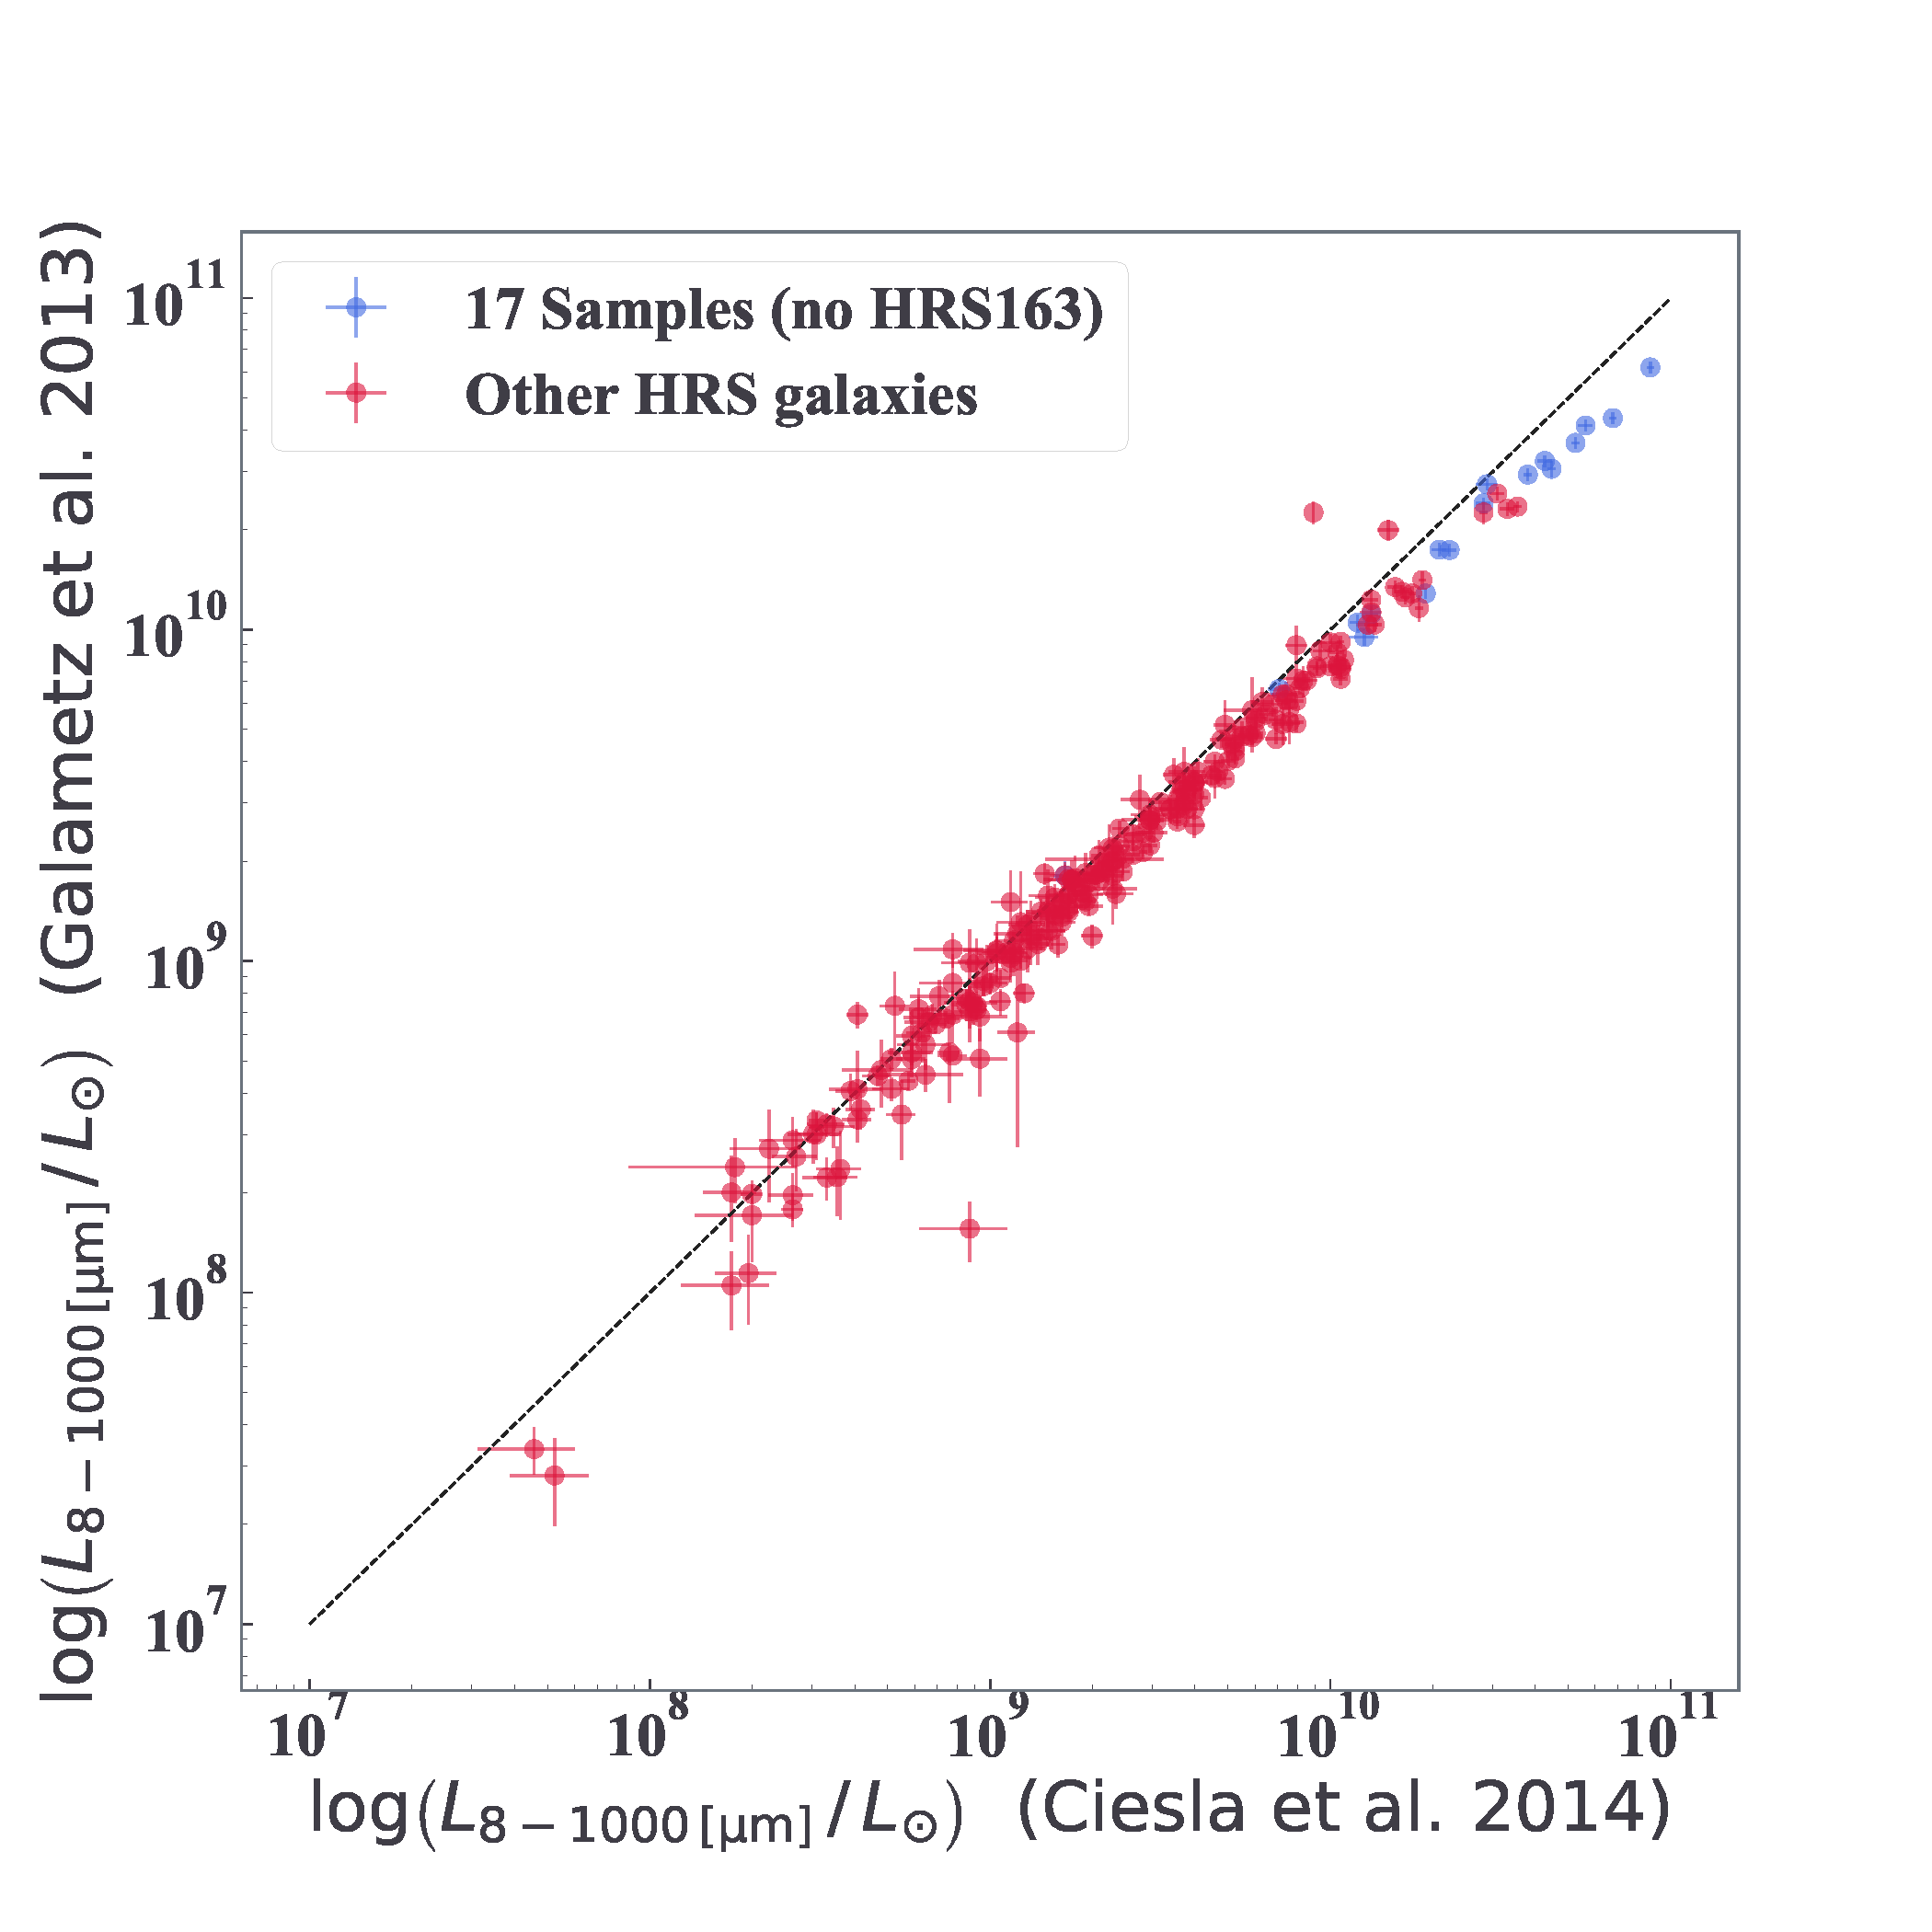
\includegraphics[width=.8\linewidth]{Chapter_4/Figures/Method_TIRcomparison.pdf}
    \caption[The comparison of total IR luminosities]{\label{fig:tircomparison}
        The comparison of total IR luminosity at $8\mbox{--}1000\micron$ from different methods.
        Here, we show all HRS galaxies which have both luminosities.
        Blue plots show galaxy samples selected in Section~\ref{sec:crossmatching} and~\ref{sec:reducegalaxysamples}, and red ones show other HRS galaxies.
        The difference of both luminosities is less than factor 2.
    }
\end{figure}

Hereafter, we use $L_{8\mbox{--}1000\mathrm{\mu m}}$ obtained here to calculate the $\qn$ parameter and SFRs.



\section{Fitting to $\qn$ Parameters}\label{sec:fittingtoq}
Here, we show how to do the fitting to $\qn$.
%If we add the chapter 2, delete after , which emitted from~~~
At low frequencies around $100\MHz$, the synchrotron radiation can be dominant, which emitted from high energy electrons accelerated by the supernova remnant.
In this paper, we assume radio emission has a single power-law on the frequency and adopt the following equation:

\begin{equation}\label{eq:q_fitting}
    q_{\nu} = -\gamma\log{\nu} + \beta
\end{equation}
where $q_{\nu}$ is defined by Equation~\ref{eq:q_def} at $\nu\MHz$, $\gamma$ is the power-law index showing the frequency dependence of $\qn$, and $\beta$ is the second fitting parameter.

In this study, we execute two types of fitting:

\begin{enumerate}
    \item Fitting to only MWA frequencies ($72\mbox{--}231\MHz$)
    \item Fitting to $1500\MHz$ besides MWA frequencies
\end{enumerate}

The flux data at $1500\MHz$ is obtained from \citet{Boselli2015}, and here we use only high-quality flux data (flag = 1 in \citealt{Boselli2015}).
These two types of fitting might allow us to judge the correctness of a single power-law assumption.
These fitting results are summarized in Section~\ref{sec:GammaDistribution}.



\section{Calculating the SFR}\label{sec:calculatingsfr}
In this Section, we describe how to derive SFR from low-frequency radio emissions.\\
Here, we estimate the radio SFR, combining Equation~\ref{eq:q_def} with the following equations:

\begin{align}
    \mr{SFR}\msb{IR} &= 3.88 \times 10^{-44}\brp{\frac{L\msb{8-1000\,\mu m}}{\mr{erg}\,s^{-1}}}\label{eq:sfrir},\\
    q_{\nu\,\mr{MHz}} &= \q{1500\MHz} + \log{\brp{\frac{\nu\,\mr{MHz}}{1500\,\mr{MHz}}}}^{\gamma}\label{eq:q_nuto1500}.
\end{align}

Equation~\ref{eq:sfrir} calculates SFR from the total IR emission in \citet{Murphy2011}, and Equation~\ref{eq:q_nuto1500} shows the difference of the $\qn$ between a certain wavelength $\nu$ and $1500\MHz$.

Substituting equation~\ref{eq:q_def} and~\ref{eq:q_nuto1500} into equation~\ref{eq:sfrir} yields the following equation to estimate SFR from the radio emission at $\nu\MHz$:

\begin{equation}\label{eq:sfrfromradio}
    \mr{SFR}_{\mr{Radio},\,\nu} = \brp{1.46\times10^{-31}} 10^{q\msb{1500\MHz}} {\brp{\frac{\nu\,\MHz}{1500\MHz}}}^{-\gamma} L_{\mr{Radio},\,\nu}.
\end{equation}

In Section~\ref{sec:sfrfromlowradio}, we show the results of calculating SFR from the low-frequency radio using this equation and comparing it with the SFR from other indicators.



%\bibliographystyle{mnras}
%%\bibliography{example} % if your bibtex file is called example.bib
%\bibliography{masterthesis}
